%! Mode:: "TeX:UTF-8"
%! TEX program = xelatex
\PassOptionsToPackage{quiet}{xeCJK}
\documentclass[withoutpreface,bwprint]{cumcmthesis}
\usepackage{etoolbox}
\BeforeBeginEnvironment{tabular}{\zihao{-5}}
\usepackage[numbers,sort&compress]{natbib}  % 文献管理宏包
\usepackage[framemethod=TikZ]{mdframed}  % 框架宏包
\usepackage{url}  % 网页链接宏包
\usepackage{subcaption}  % 子图宏包
\newcolumntype{C}{>{\centering\arraybackslash}X}
\newcolumntype{R}{>{\raggedleft\arraybackslash}X}
\newcolumntype{L}{>{\raggedright\arraybackslash}X}


%%%%%%%%%%%%%%%%%%%%%%%%%%%%%%%%%%%%%%%%%%%%%%%%%%%%%%%%%%%%%
% 论文标题
\title{量子近似优化算法QAOA中的最优初始化参数}


%%%%%%%%%%%%%%%%%%%%%%%%%%%%%%%%%%%%%%%%%%%%%%%%%%%%%%%%%%%%%
%% 正文
\begin{document}

\maketitle
\begin{abstract}
在量子近似优化算法 (QAOA) 中,变分量子线路初始参数的选择会极大影响迭代优化的效率。
本赛题要求选手给出一个算法,对任意给定 QAOA 线路给出一组初始化参数,使得初始状态下目标函数尽可能小。
本文以一份预制的最优参数表为基础,对其进行多策略的微调训练,可进一步降低标准QAOA线路初始状态下的期望值。
该方法训练所得的预制表可进一步通过线性插值的方法,外推到训练集中未见过的其他线路深度的情况。
实验表明,我们所提出的方法最终得分 30641.0100,超过基线方法 22.56\%。

\keywords{量子近似优化算法 \quad QAOA \quad 参数初始化 \quad 最优化问题 }
\end{abstract}


%%%%%%%%%%%%%%%%%%%%%%%%%%%%%%%%%%%%%%%%%%%%%%%%%%%%%%%%%%%%%
% 目录
% \tableofcontents
% \newpage


%%%%%%%%%%%%%%%%%%%%%%%%%%%%%%%%%%%%%%%%%%%%%%%%%%%%%%%%%%%%%
\section{问题背景}

量子近似优化算法 (QAOA) 是含噪中等规模量子计算机时代最具有应用潜力的变分量子算法之一,可用于高效地近似求解诸如
图最大割 (MaxCut) 与最小割 (MinCut)、二次无约束二元优化问题 (QUBO)、Ising-模型 等被证明为 NP-Hard 的离散组合优化问题,
或用于线性系统求解 (Linear-system Solver) 的加速。
QAOA通过迭代优化一个变分量子线路,最小化系统哈密顿量的期望,来近似模拟量子绝热演化过程,制备含有目标解信息的末态。
其中变分量子线路初始参数的选择会极大影响之后迭代优化过程的效率,乃至最终收敛到解的解的质量。
因此,线路初参选择是本领域中一个重要的讨论课题。


%%%%%%%%%%%%%%%%%%%%%%%%%%%%%%%%%%%%%%%%%%%%%%%%%%%%%%%%%%%%%
\section{问题分析}

\begin{figure}
	\centering
	\subcaptionbox{k阶Ising模型\label{fig:ising}}
	{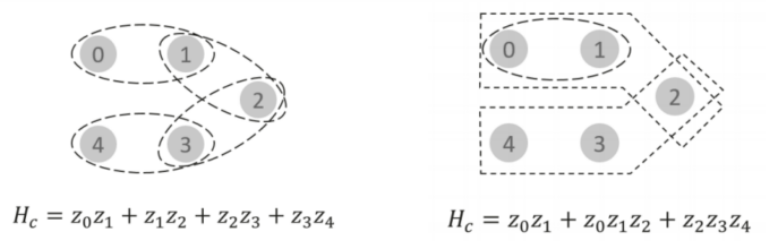
\includegraphics[width=0.45\textwidth]{figures/ising_model.png}}
	\subcaptionbox{标准QAOA线路\label{fig:qaoa}}
	{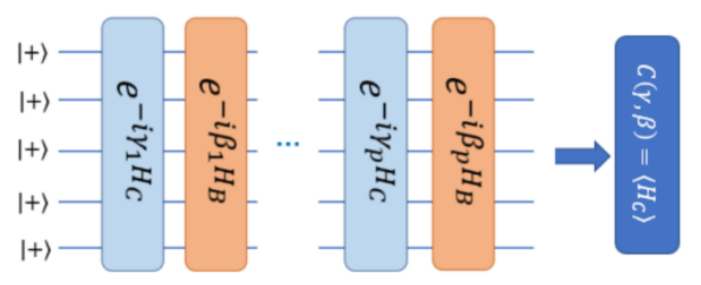
\includegraphics[width=0.45\textwidth]{figures/qaoa_circ.png}}
	\caption{Ising模型及其对应的QAOA线路}
	\label{fig:ising-qaoa}
\end{figure}

本赛题要求选手给出一个变分线路参数初始化方案,对于任意给定的带权重高阶 Ising 模型所对应的标准 p-层 QAOA 线路,如图 \ref{fig:ising-qaoa} 所示,
给出线路的初始参数 $ \gamma_p $ 和 $ \beta_p $ ,使得线路在迭代优化之前的初始状态下的目标函数尽可能小。

在目前相关工作中,对于此初参选择问题的主要方案是参数转移,即依据类比逻辑和损失函数地形图的拓扑相似性,将已知问题设置的最优参数经过一定的规则放缩从而转移到到新的问题设置情况。
例如,文献 \cite{Basso2022} 提供了一张预制表,给出了在图的度数 $ D \rightarrow \inf $ 情况下无权图的 MaxCut 问题所对应 QAOA 线路层数从 p=1 到 p=17 的最优线路参数 $ \gamma^\mathrm{inf} $ 和 $ \beta^\mathrm{inf} $。
文献 \cite{Shaydulin2023} 提出公式 \ref{eq:gamma-23} 来对此预制表中的 $ \gamma^\mathrm{inf} $ 参数进行放缩变换得到 $ \gamma^\ast $,以迁移应用到带权图 MaxCut 问题的情况。
文献 \cite{Sureshbabu2024} 进一步将其改进为公式 \ref{eq:gamma-24},优化了初参质量,极大了降低后续线路优化所需的迭代次数。

\begin{equation}
\gamma^\ast = \frac{\gamma^{\mathrm{inf}}}{\frac{1}{|E|} \sum_{\{u,v\} \in E} |w_{uv}|} \mathrm{arctan}(\frac{1}{\sqrt{D-1}})
\label{eq:gamma-23}
\end{equation}

\begin{equation}
\gamma^\ast = \frac{\gamma^{\mathrm{median}}}{\sqrt{\frac{1}{|E|} \sum_{\{u,v\} \in E} w_{uv}^2}} \mathrm{arctan}(\frac{1}{\sqrt{D-1}})
\label{eq:gamma-24}
\end{equation}


%%%%%%%%%%%%%%%%%%%%%%%%%%%%%%%%%%%%%%%%%%%%%%%%%%%%%%%%%%%%%
\section{解决方案}

我们的解决方案主要包含三部分:为上述 $ \gamma $-迁移变换公式引入重缩放因子、对预制表进行多策略的微调训练、线性插值外推方案。

\subsection{重缩放因子}

观察到公式 \ref{eq:gamma-23} 和公式 \ref{eq:gamma-24} 的分子 $ \gamma^\mathrm{inf} $ 和 $ \gamma^\mathrm{median} $ 是相近的,核心差异主要在分母不同:
文献 \cite{Shaydulin2023} 使用了 $ L_1 $ 距离,而文献 \cite{Sureshbabu2024} 使用了 $ L_2 $ 距离。
我们没有尝试别的闵可夫斯基 $ L_p $ 距离, 但受此启发,我们在公式 \ref{eq:gamma-24} 的基础上,引入一个乘性的全局常量因子 $ \mathrm{rescaler} $ 来作整体调控,
并且使用 $ \gamma^\mathrm{inf} $ 来替换 $ \gamma^\mathrm{median} $,最终如公式 \ref{eq:gamma-ours} 所示。

\begin{equation}
\gamma^\ast = \mathrm{rescaler} * \frac{\gamma^{\mathrm{inf}}}{\sqrt{\frac{1}{|E|} \sum_{\{u,v\} \in E} w_{uv}^2}} \mathrm{arctan}(\frac{1}{\sqrt{D-1}})
\label{eq:gamma-ours}
\end{equation}

\subsection{多策略微调预制表}

观察到文献 \cite{Shaydulin2023} 和文献 \cite{Sureshbabu2024} 都只对 $ \gamma $ 作了迁移变化,对于 $ \beta $ 参数仍然直接沿用了文献 \cite{Basso2022} 预制表中的 $ \beta^\mathrm{inf} $,这或许是一个可以优化的点。
另一方面,文献 \cite{Basso2022} 给出的最优初参在 p=4,8 的情况下可如图 \ref{fig:theta0} 所示:左半递增部分是 $ \gamma^\mathrm{inf} $,右半递降部分是 $ \beta^\mathrm{inf} $ 参数。
这些变化曲线的趋势和我们所见在一些量子绝热演化应用 \cite{An2022} 中所设计的哈密顿量调度函数(如图 \ref{fig:schedulers}所示)曲线有些不太一致,
即不太满足 $ \gamma $ 曲线单增,且其导函数单减的性质,这可能也是一个可以改进的方面。

\begin{figure}
	\centering
	\subcaptionbox{预制表参数 (p=8)\label{fig:theta0}}
	{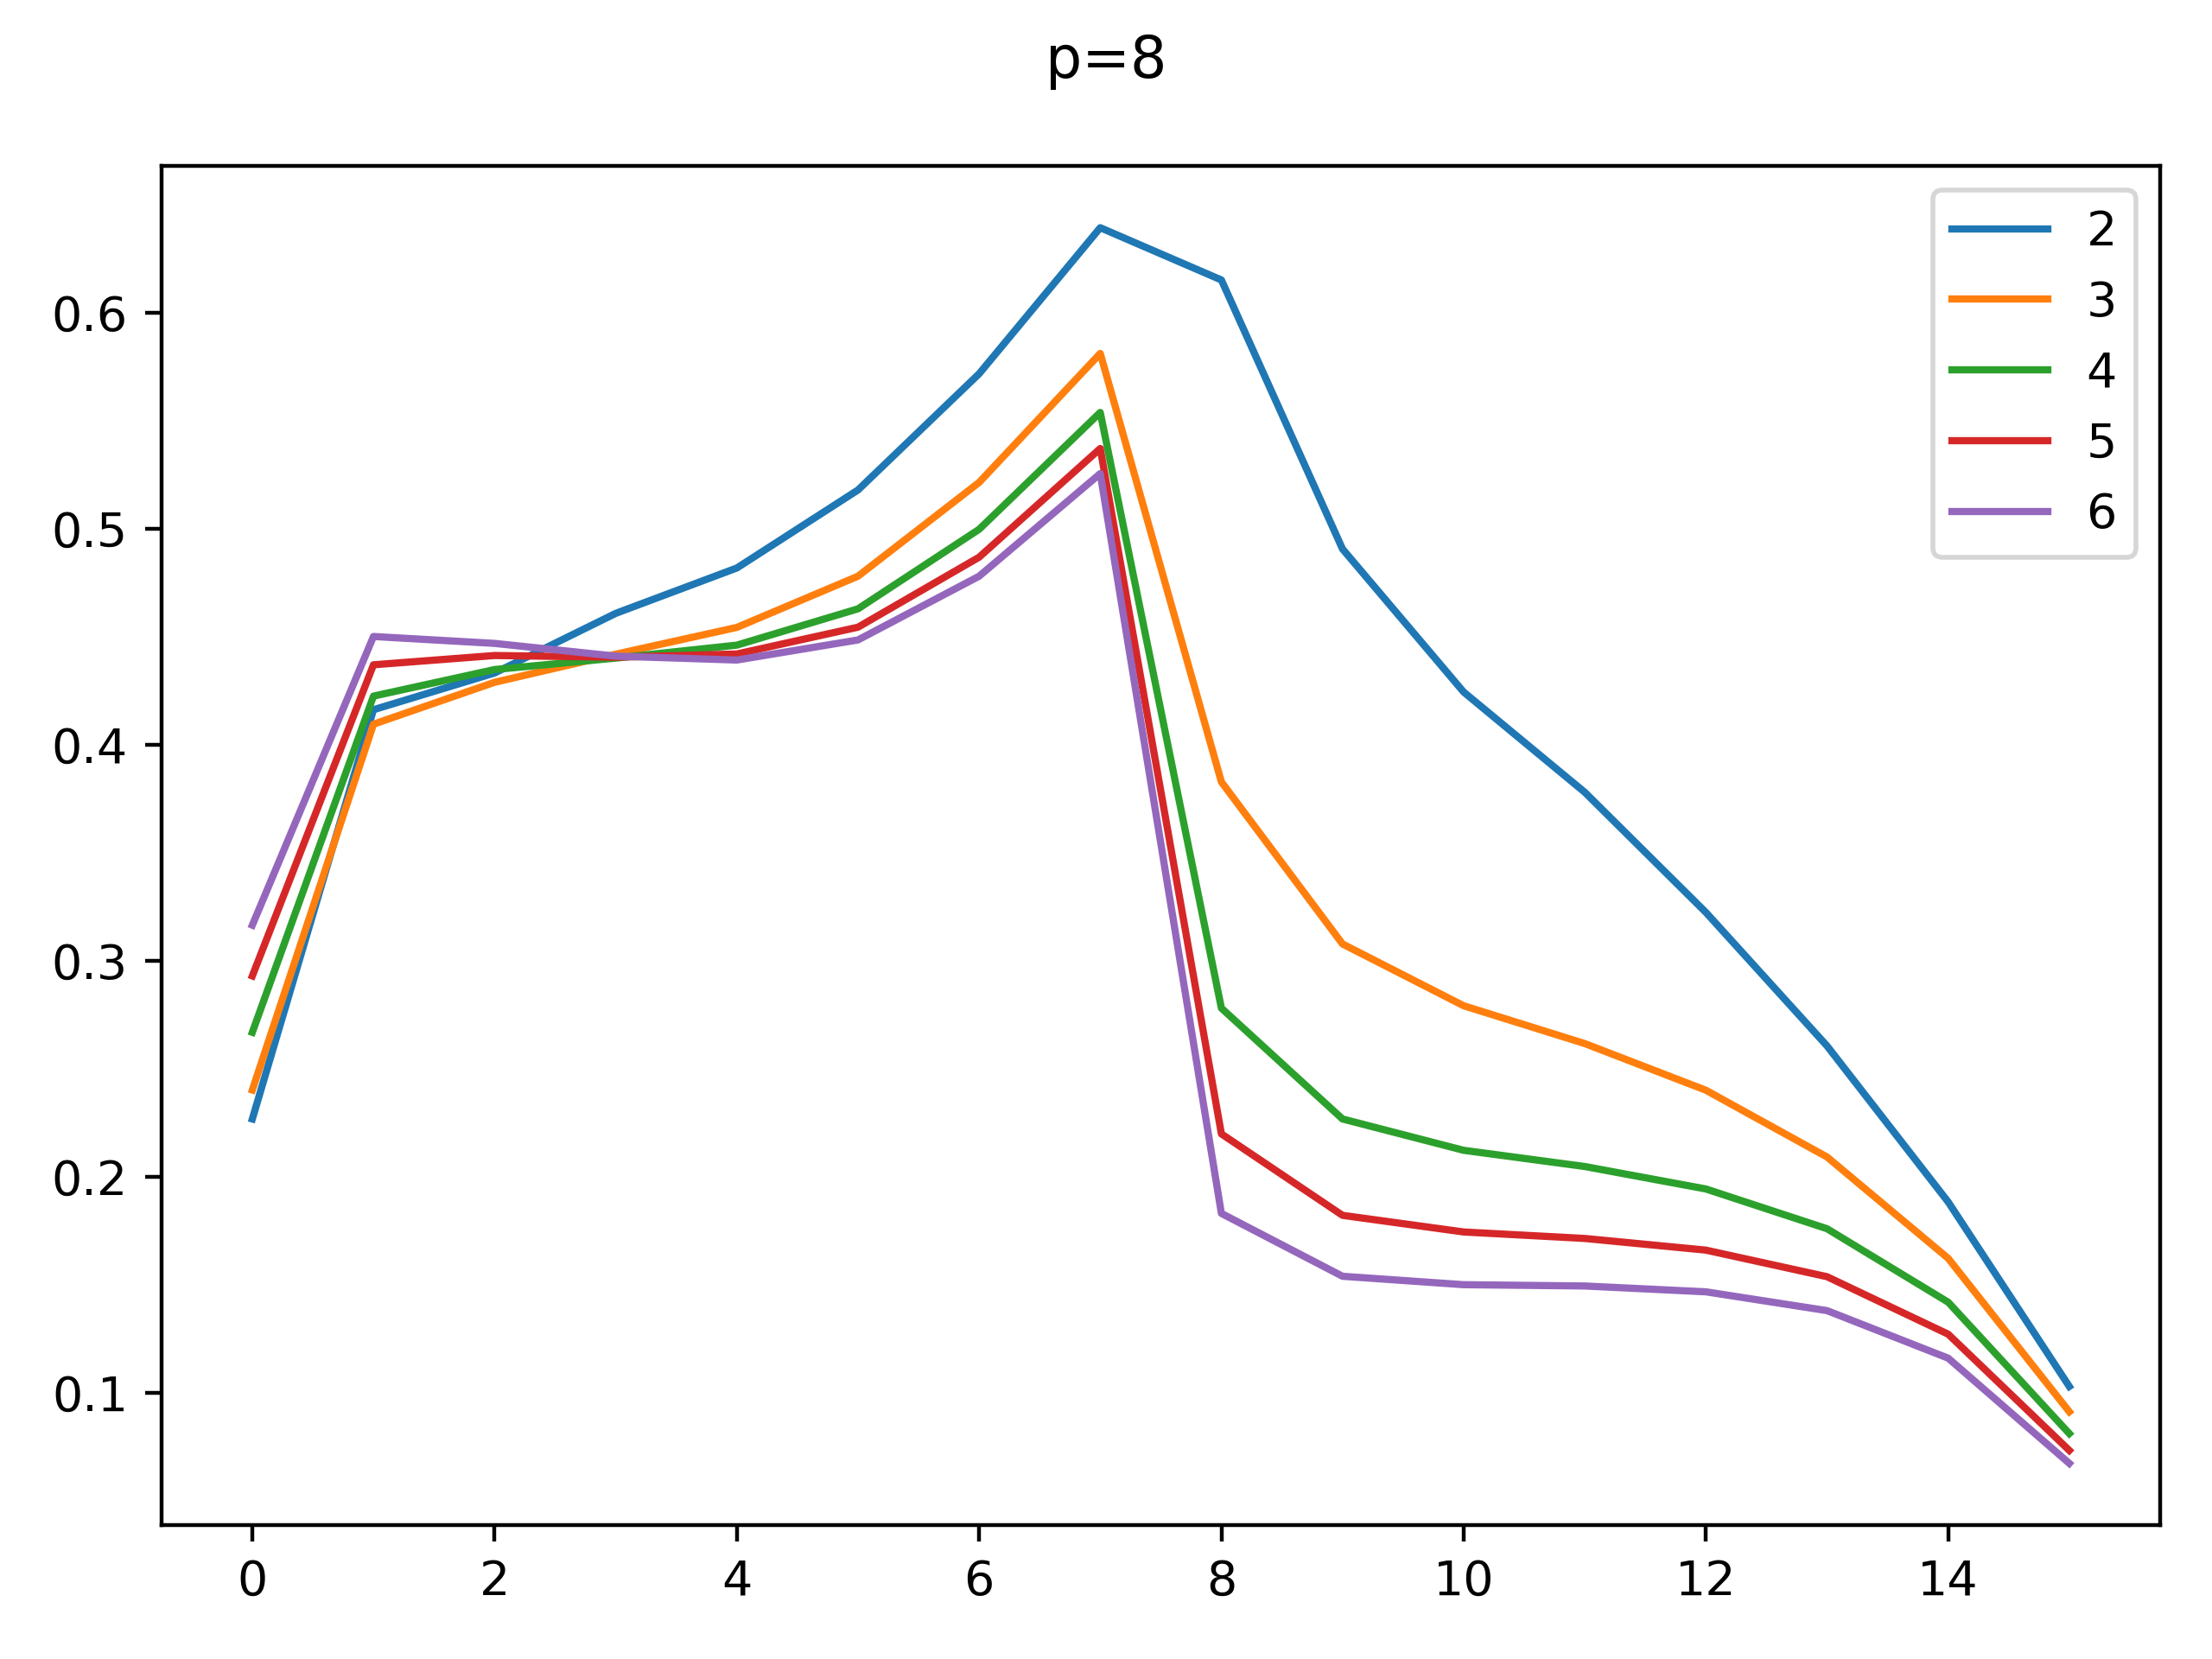
\includegraphics[width=0.45\textwidth]{figures/original_p=8.png}}
	\subcaptionbox{哈密顿量调度函数\label{fig:schedulers}}
	{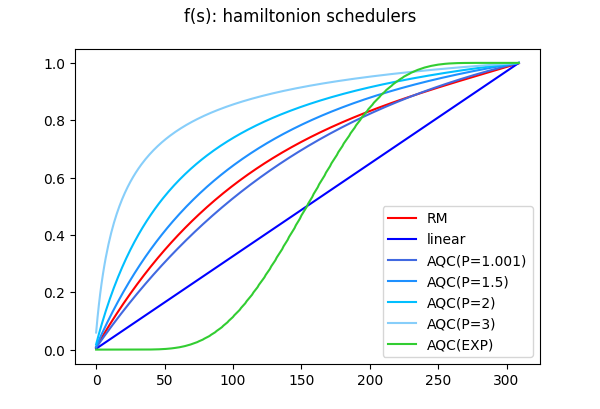
\includegraphics[width=0.5\textwidth]{figures/schedulers.png}}
	\caption{预制表参数与哈密顿量调度函数}
\end{figure}

综合上述两点,我们采用微调训练的方式进一步优化预制表中的参数 $ \gamma^\mathrm{inf} $ 和 $ \beta^\mathrm{inf} $,即使用各具体样本的最优参数来调整全局平均最优参数。
最朴素的更新策略如公式 \ref{eq:update0} 所示,其中 $ \theta_i^\ast $ 为第 $ i $ 次训练迭代后的全局平均最优参数,而 $ \hat{\theta_i} $ 为第 $ i $ 次训练时所用样本的最优参数, $ \Delta x $ 可理解为学习率。

\begin{equation}
\theta_{i+1}^\ast = (1 - \Delta x) * \theta_i^\ast + \Delta x * \hat{\theta_i}
\label{eq:update0}
\end{equation}

为了获得更好的训练效果,我们进一步引入了学习率衰减、自适应损失、差分动量的更新策略,此时策略的更新公式变为 \ref{eq:update1}。
其中 $ \Delta x $ 依然为基准学习率;$ w $ 为学习率衰减因子,受到迭代次数的累计而减小;
$ \Delta E $ 为各样本优化前后的能量值之差,来对数尺度地放缩学习率,使得能量值差越大的样本的个体参数才能对全局参数产生足够大影响;
而 $ \mu_i^\ast $ 为第 $ i $ 此迭代时累计产生的最优参数的动量,$ m $ 为动量平衡因子,这变相实现了小批次平均的梯度下降,保证了训练过程的稳定。
最后,观察到无权图和带权图在数据分布上的显著不一致,我们认为使用同一张预制表来应对两种情况可能会导致一些模型建模内在的矛盾。
所以我们以图权值的方差是否超过特定阈值为判据,为近似无权图和带权图分别建立一套预制表,这就是无权-带权分离建模策略。

\begin{equation}
\begin{split}
\Delta E &= E_{\mathrm{before}} - E_{\mathrm{after}} \\
\tilde{\Delta x} &= \Delta x * (w^{\frac{\mathrm{cur\_iter}}{\mathrm{decay\_per\_iter}}}) * \mathrm{log}(1 + \Delta E) \\
\mu_{i+1}^\ast &= (1 - m) * \mu_i^\ast + m * \hat{\theta_i} \\
\theta_{i+1}^\ast &= (1 - lr) * \theta_i^\ast + \tilde{\Delta x} * \mu_{i+1}^\ast \\
\end{split}
\label{eq:update1}
\end{equation}

\subsection{线性插值外推}

预制表是针对特定层数 p=4,8 的QAOA线路进行建模的,当目前线路为其他层数时,可以使用如图 \ref{fig:expolate} 所示的线性插值外推来获得次优初参。
以 6 层为例,首先将已建模的层数 p=4 (蓝色) 和 p=8 (橙色) 的最优参数进行长度对齐,然后求平均得到 fused (绿色) 参数,最后将其以首尾为锚点等比例线性拉伸为目标参数长度,保持轮廓一致性。
须注意该方法不只对于内插值有效,小于 4 层或大于 8 层的操作流程也完全一致。

\begin{figure}[h!]
	\centering
	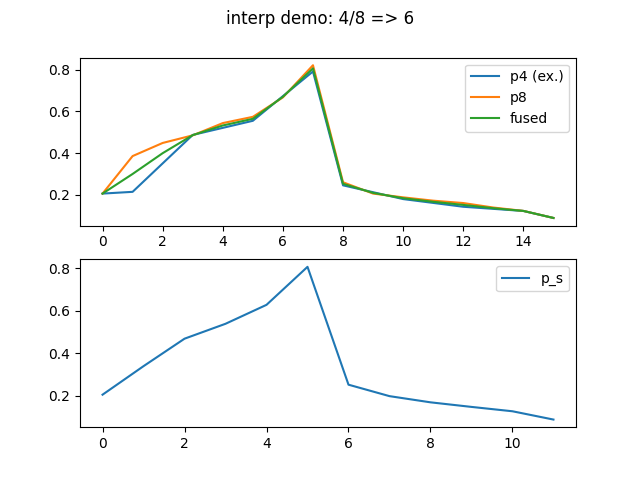
\includegraphics[scale=0.6]{figures/interp.png}
	\caption{最优参数预制表的线性插值外推}
	\label{fig:expolate}
\end{figure}


%%%%%%%%%%%%%%%%%%%%%%%%%%%%%%%%%%%%%%%%%%%%%%%%%%%%%%%%%%%%%
\section{结果}

我们使用 Adam 优化器进行 QAOA 线路的优化,在赛题给出的数据集上训练每个样本 100 步 (fast 模式下仅训练 40 步)。
其他超参设置为 $ lr = 1e-5, \Delta x = 0.1, w = 0.98, \mathrm{decay\_per\_iter} = 100, m = 0.6 $。
实验结果如表 \ref{tbl:result} 所示,简要介绍如下:

\begin{itemize}
\item 方法 \#1 和 \#2 为基线,其中 \#2 为比赛模板代码给出的标准基线,而\#1 为其前作基础,可见距离函数的选择对性能影响巨大
\item 方法 \#3 在标准基线 \#2 的基础上仅仅调整了 rescaler 就导致了 8.87\% 的分数提升,说明了该参数对样本共性的重要影响
\item 方法 \#4 为朴素的优化-平均,即对所有样本各自求得最优参数后作简单平均。这引起了 12.04\% 的分数提升,说明样本间差异也是重要的考虑因素
\item 方法 \#5 为朴素的微调,即对预制表按公式 \ref{eq:update0} 进行迭代优化,它只比 \#4 略好一些
\item 方法 \#6 $ \sim $ \#10 为本文提出的多策略微调算法,即对预制表按公式 \ref{eq:update1} 进行迭代优化
\begin{itemize}
  \item 方法 \#6 $ \sim $ \#10 均引入了损失值自适应策略,抑制恶劣样本产生的负面影响
  \item 方法 \#7 $ \sim $ \#9 引入了学习率衰减策略,确保微调过程能呈现为收敛态势
  \item 方法 \#8 $ \sim $ \#10 引入了差分动量策略,可使用更少的优化步数以节省时间
  \item 方法 \#10 \ 在 \#9 的基础上引入了均权-加权分离的策略,并在此配置下达到了我们的最高分 30641.0100,相对于标准基线提升了 22.56\%
  \item 注意到方法 \#9 和 \#10 都重新调整了重缩放因子,是因为经过优化的新参数已经偏离了原始的位置,为了适应新的方差必须重新确定;
            而在 \#10 中去掉了学习率衰减策略,是因为此时平均损失值已经很小了,再作放缩将无法推动学习
\end{itemize}
\end{itemize}

\begin{table}[h!]
	\centering
	\caption{实验结果}
	\begin{tabular}{llll}
		\textbf{\#} & \textbf{local score} & \textbf{submit score} & \textbf{comment} \\
		\hline
		\#1 & 11730.14583 & 16627.4960 &  PT-WMC \cite{Shaydulin2023} , reference  \\
		\#2 & 16526.79871 & \underline{24999.9025} & PS-WP \cite{Sureshbabu2024} , baseline  \\
		\#3 & 17816.62534 & 27217.3001 & baseline; rescaler=1.275  \\
		\#4 & 18516.17254 &         -          & opt-avg  \\
		\#5 & 18535.15152 & 27998.4487 & ft; rescaler=1.275 \\
		\#6 & 20489.27983 & 29920.0329 & ft-ada; rescaler=1.275  \\
		\#7 & 20948.34952 & 30332.7544 & ft-ada-decay; rescaler=1.275  \\
		\#8 & 20381.14635 & 29800.8173 & ft-ada-decay-moment-fast; rescaler=1.275 \\
		\#9 & 21033.52542 & 30264.7276 & ft-ada-decay-moment-fast\_ft; rescaler=1.165  \\
		\#10 & 21432.33415 & \textbf{30641.0100} & ft-ada-moment-fast\_ft-ex; rescaler=1.165 \\
	\end{tabular}
	\label{tbl:result}
\end{table}

微调优化后的预制表参数如图 \ref{fig:theta1} 所示,可见左半 $ \gamma $ 部分已满足函数单增且导函数单减的性质,符合我们在量子绝热演化应用中的相应观察。
NON\_EQ 和 SIM\_EQ 分别对应于带权图和近似无权图的预制表,在此图示中看不出显著的差异,但各数值上确有 $ 0.001 \sim 0.1 $ 量级的均值偏差。

\begin{figure}
	\centering
	\subcaptionbox{层数 p=4}
	{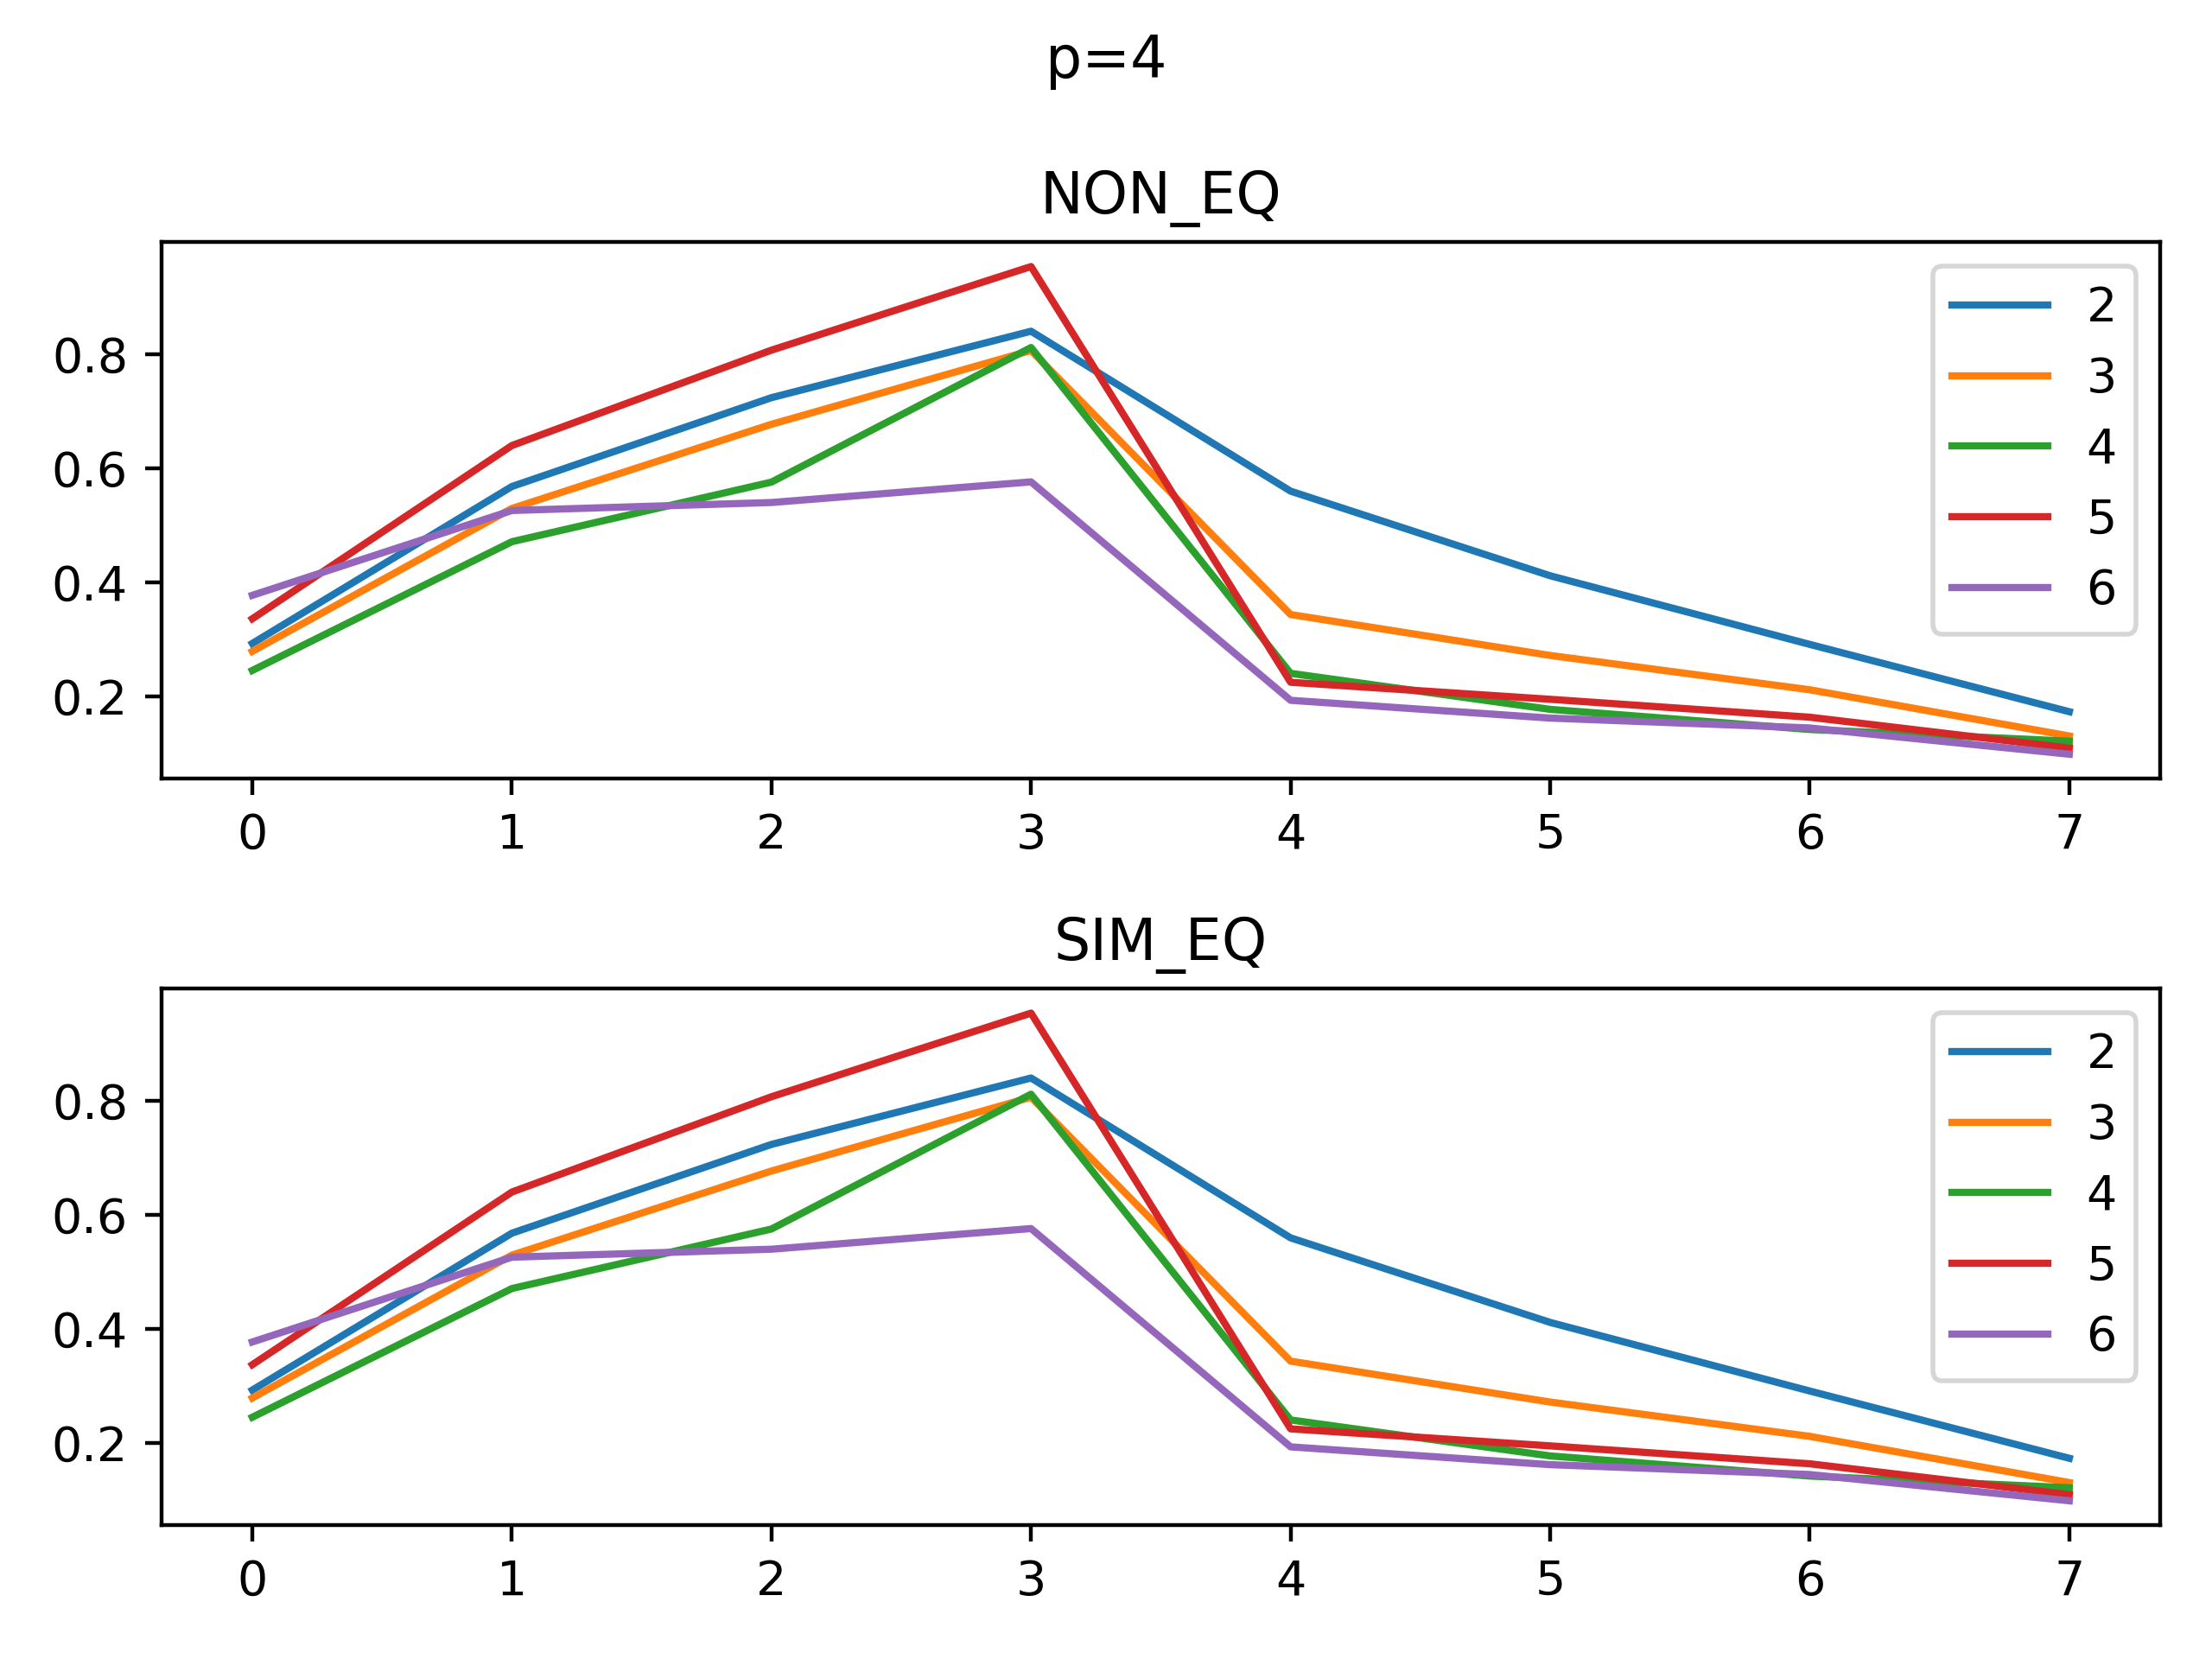
\includegraphics[width=0.48\textwidth]{figures/p=4.png}}
	\subcaptionbox{层数 p=8}
	{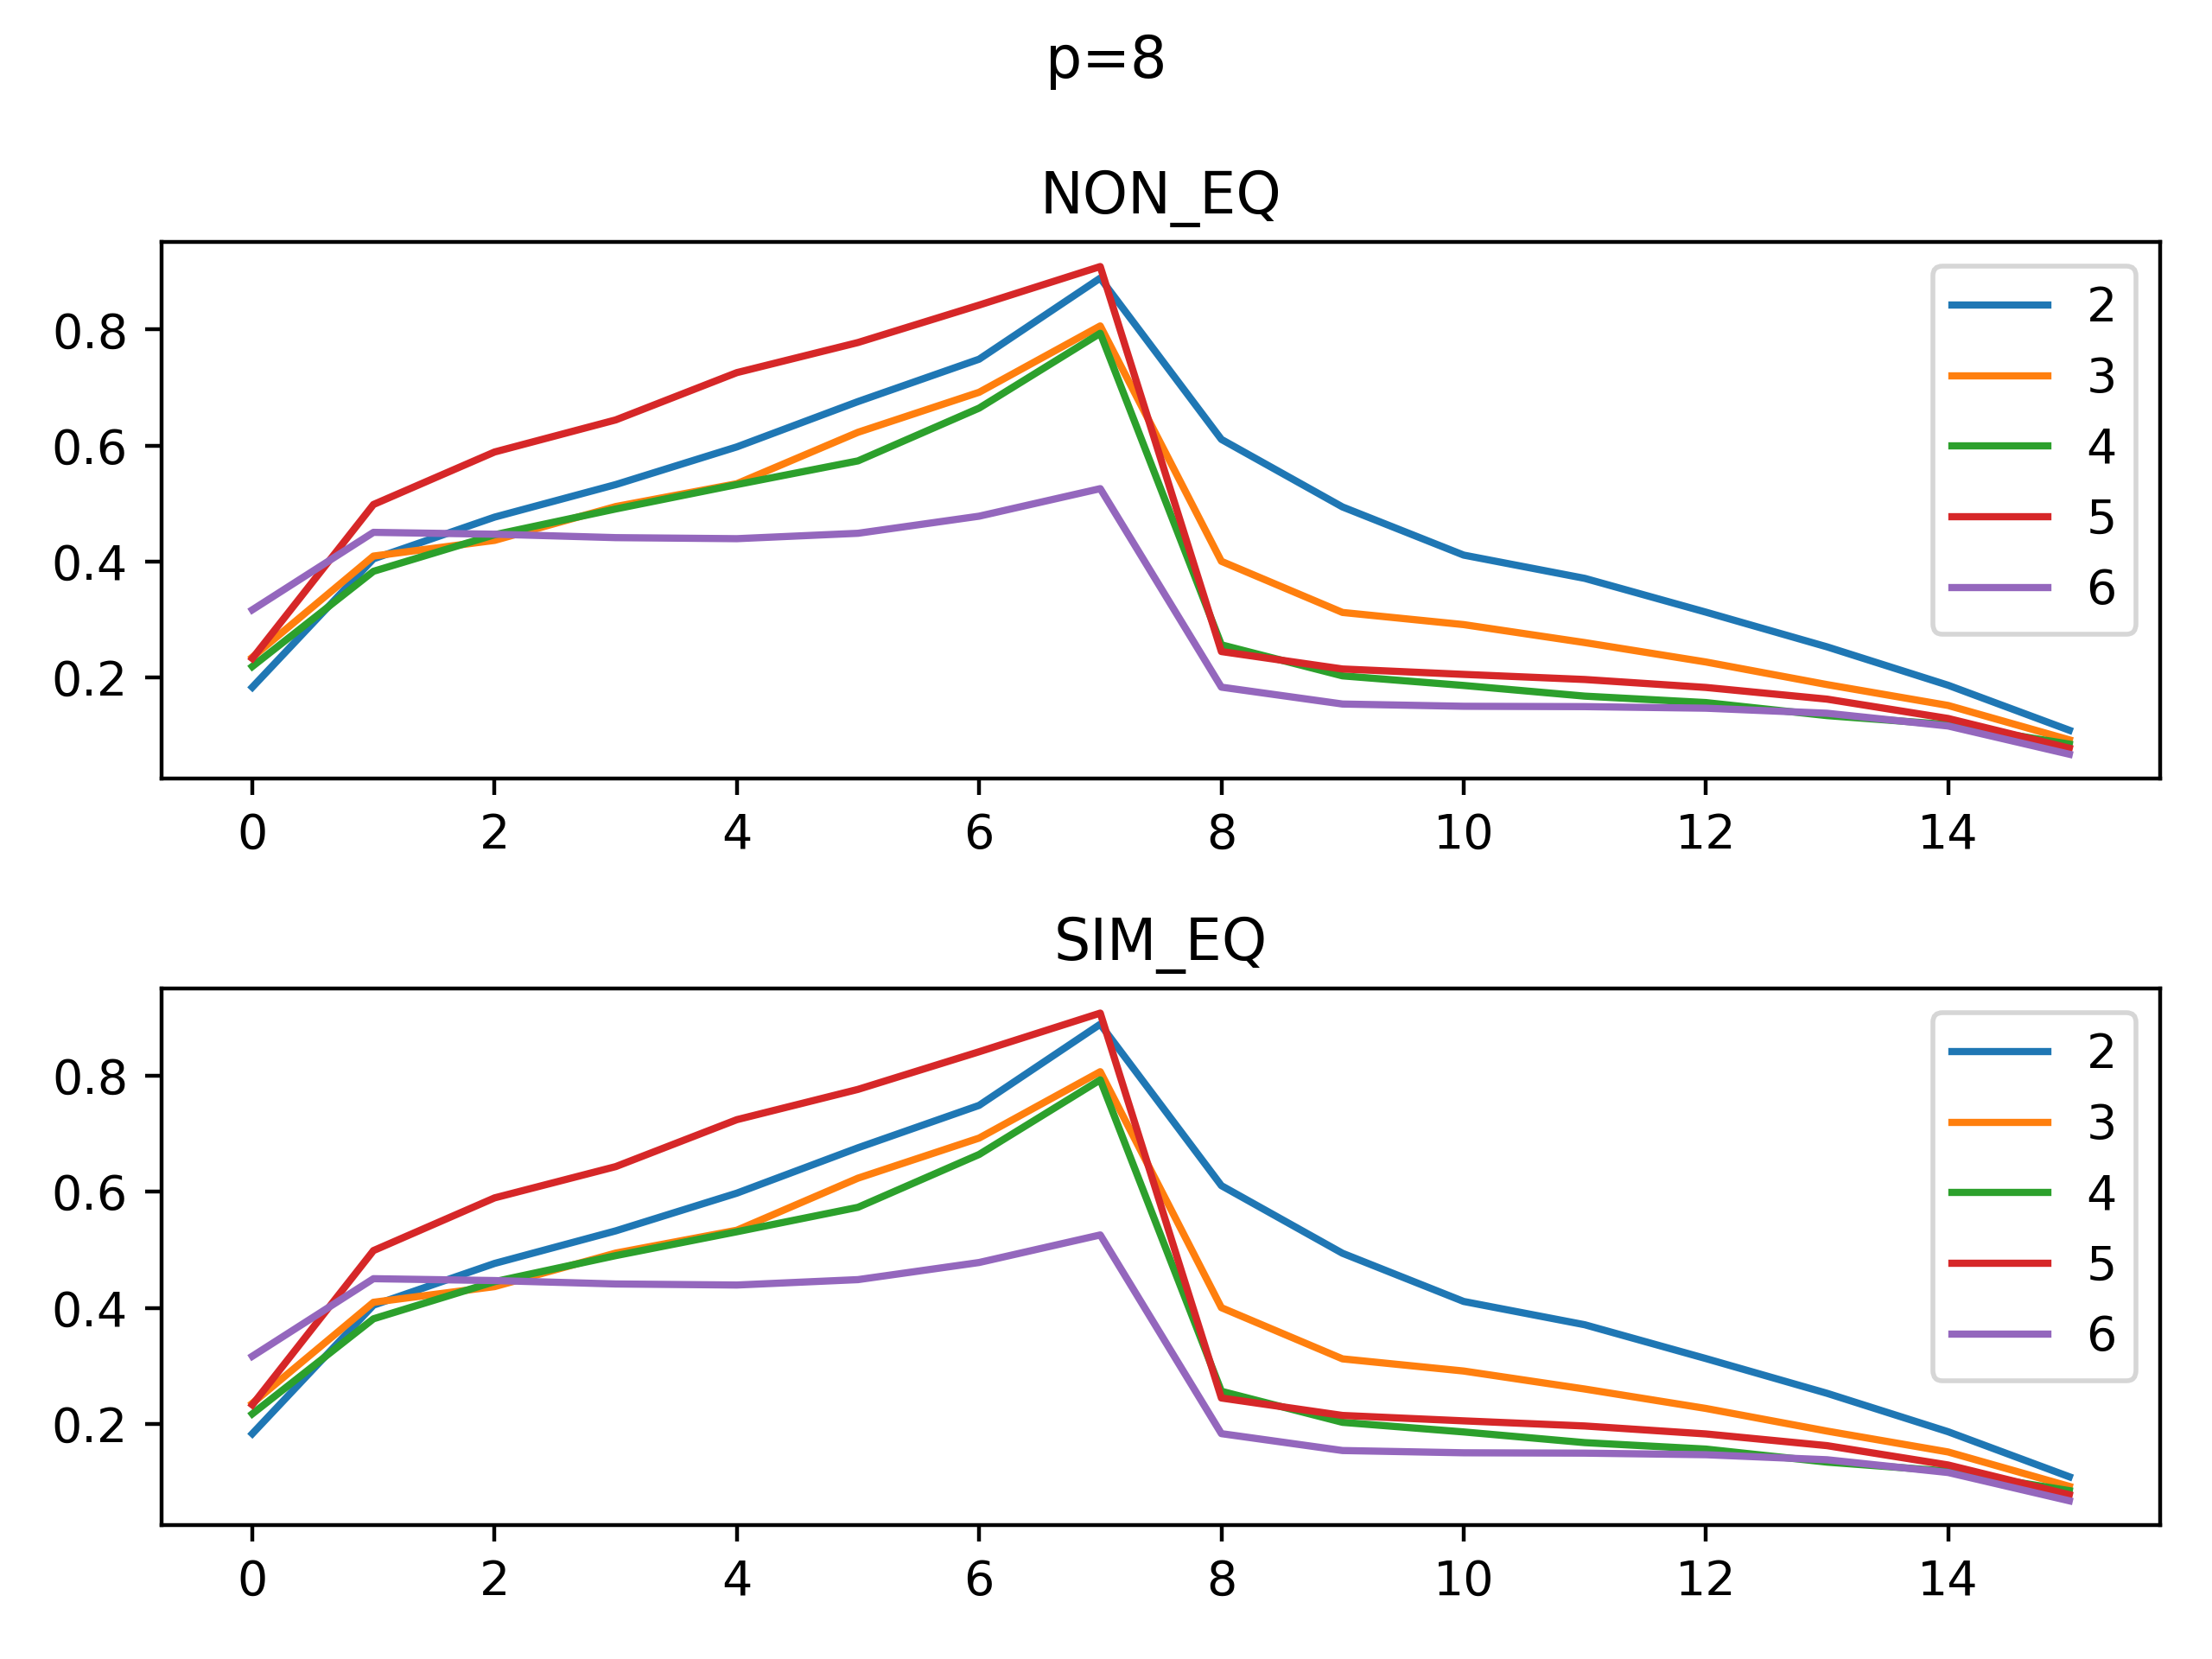
\includegraphics[width=0.48\textwidth]{figures/p=8.png}}
	\caption{微调优化后的预制表参数}
	\label{fig:theta1}
\end{figure}


%%%%%%%%%%%%%%%%%%%%%%%%%%%%%%%%%%%%%%%%%%%%%%%%%%%%%%%%%%%%%
\section{总结及展望}

针对QAOA线路最优初参选取问题,本文提出了一种基于预制表进行多策略微调的方法,进一步降低了线路初始损失值,为后续迭代优化创造有利起点。
提出了一种线性插值外推的方式,可在保持参数数值比例一致的条件下进行内外插值,以扩展训练优化后预制表的应用范围。

在比赛数据集上的进一步的实验表明,我们所提方法能达到的最好表现,仍然距离每个样本被优化到各自最优解这种完美情况仍有 10\% 的差距,
这或许表明了此系列方法还有长足的改进空间,亦或许暗示了这个问题本身的复杂,即仍然存在某些各向异性的因素,很难通过统计建模去总体性地刻画。
未来的工作或将向着离群性样本,奇异点和相变的方向讨论和发展。


%%%%%%%%%%%%%%%%%%%%%%%%%%%%%%%%%%%%%%%%%%%%%%%%%%%%%%%%%%%%%
%% 参考文献
\nocite{*}
\bibliographystyle{gbt7714-numerical}  % 引用格式
\bibliography{ref.bib}  % bib源


%%%%%%%%%%%%%%%%%%%%%%%%%%%%%%%%%%%%%%%%%%%%%%%%%%%%%%%%%%%%%
%% 附录
\newpage
\begin{appendices}

\section{主要代码}

预制表的微调训练流程:

\lstinputlisting[language=python]{code/opt.py}

预制表的查表方法:

\lstinputlisting[language=python]{code/query.py}

\end{appendices}
\end{document}